\documentclass[a4paper,12pt,twoside]{book}
\usepackage[english]{babel}
\usepackage{blindtext}
\usepackage[utf8]{inputenc}
\usepackage{amsmath}
\usepackage{apacite}
\usepackage{natbib}
\usepackage{listings}
\usepackage{graphicx}

\bibliographystyle{apacite}
\pagestyle{myheadings}

\title{Analyzing opportunities arround city traffic optimization }
\author{Toma Becea}

\begin{document}

\maketitle

\clearpage

\section{Introduction}

The traffic in a city is a very complex phenomenon. The parties involved are of many types: cars, pedestrians, buses, trams, taxi cabs (they are arugably cars, too but there might be small differences, e.g. they are allowed to drive on public transport lanes), bicycles, e-scooters (again, they are arguably same as bicycles), etc. Then there are rules on how they move: traffic lights for cars in junctions, across roads for pedestrian crossings, different traffic lights for buses and trams, etc. Within this rule-bounded context is the free will of every intelligent decision maker (it might be a human or it might be a self driving car with algorithms which we can deem as being intelligent from the perspective of behaving and moving within the traffic), the individual randomness unified into a collective orderness.

But the devil is in the details: the orderness we see when looking across the entire city uncovers many opportunities. The architecture of many old cities is not meant for current traffic needs. The behavior of residents and dwellers of a city is not optimized for collective good but for personal comfort. The heterogenous and continous development of a city might add pain to the picture. Highly-accelerated developing areas or neighborhoods pose problems which city administrations are slow to understand and tackle with. Those, so far, are problems on the macro scale of a spectrum. On the other side of the spectrum, called micro, we can find another set of opportunities which can be modeled and analyzed through computer based simulations. Junction design, traffic lights programming and synchronization, pedestrian crossings and their influence on the surrounding driving lanes, bus stops and their influence, side walks design, lanes formation and one way drives, etc. Those are localized problems, focused on small geographical areas.

The current chapter aim to find and define technical means on exploring intricacies within the traffic of a city. Software simulation is a broad term which encompasses any idea or way of using a computer to mimic as closely as possible a real phenomenon, with or without the help of a mathematical apparatus. This entire chapter is centered around various tehniques of using a computer for traffic simulation. There are a number of existing solutions to simulating traffic using software abilites, on various places on the macro-micro spectrum, as well as on other spectrums like discrete event vs continous simulation. Those will be explored and briefly categorized.

\section{Abstract}

The current chapter is aiming to propose a novel solution for simulating traffic in a city and exploring the opportunities which this solution makes possible to address. To describe it in few words, before going in full details on it during section \ref{sec:microservicesbasedapproachtrafficsim}, it is a discretes event based simulation, using a distributed microservices architecture where actors (defined as independent and intelligent participants in a traffic) are moving across a city and interacting with one another. They are a number of different instances running in isolation as containers. Their interaction is made via a single instance, called city simulator, which keep various statistics about the actors which are live and moving. On top of those there are few other supporting utilities, not essential for the current subject but mandatory for the simulation to run. They are a map and routing service which offers a route between two points of a city to those actors which need it and a service which renders a web page with the map of the city where the simulation takes place and the gradual occupation of its streets.

The second area of this chapter is to analyze opportunities for optimizing the traffic within a city using the aforementioned simulation solution. Those ideas will revolve around the core concepts which form the foundation of the microservices based approach for traffic simulation: discrete and independent actors (also randomness is included into their behavior), decoupled in their logic and choice, interacting via discrete events based on their selfish interest (their behiavor which this simulation is modeled for is their interest in navigating their route as fast as they can, using the shortest path between two points, departure and arrival ones).

Following concepts will be discussed in order to explore the opportunities for optimizing the traffic in a city. They are to be found in section \ref{sec:citytrafficoptimizations} and a brief list of them is presented here:

\begin{itemize}
    \item Modeling various actors with very different behaviors. For example a pedestrian and a city bus. Or a bicycle and a garbage truck.
    \item Modeling various relations between different actors. An example of such a relation can be contained actors: a pedestrian can take a tram.
    \item Introducing exception actors and their influence in the surrounding traffic. Firefighters truck moving throughout the city is one example. Cars stopped on the road is another.
    \item Localize hot areas or bottlenecks of a city: junctions, streets, bridges.
    \item Computation of various numbers and statistics. Few examples: average speed on street intervals, cars density per area and/or time.
    \item Introduce geographical differences in simulation and study their influence: a roundabout instead of a junction, a new lane on a street.
\end{itemize}

%\section{Current state of traffic simulation}

\section{A microservices based approach for traffic simulation}
\label{sec:microservicesbasedapproachtrafficsim}

\subsection{Prerequisites}
\label{subsec:prerequisites}
In order to discuss how a discrete-based, microservices architectured simulation works, few prerequisites are needed to set the base.

First definition we need is for setting the fact that we are using geographical coordinate system. It doesn't matter which one, what it matters is that all actors are using the same set of geographical coordinates and same projection (or to know if there should be a conversion). For example, they could be EPSG:4326 or EPSG:3857. To define this in an appropiate way, equation \ref{eq:coordinates} will be used. Its loosness allow any implementation to treat coordinates using a built in language data type (e.g. \textit{double} in C\#).

\begin{equation}
\label{eq:coordinates}
    C = \{ c | c \in \Re, c \geq 0 \}
\end{equation}

Simulation wise, actors do not have any \textit{intent}. They are just \textit{dumb} programs which need to be programmed to have any small \textit{intention}. To give them a \textit{sense} of selfishness they are programmed to navigate between two random points. Therefore points need to be defined as a pair of coordinates. The implementation of this will have to take care of their order or of knowing which one represents latitude and which one longitude. Equation \ref{eq:coordinatespair} defines such a pair of coordinates. Furthermore we define a way which introduce randomness into an actor's behavior: the random choice of two points. The actor needs to have two points predefined, $Pd_1$ and $Pd_2$. Those are treated as an aproximative rectangular area, out of which other two points will be randomly chosen: $Pr_1$ and $Pr_2$. Equation \ref{eq:funcrandom} defines this function, without entering into the details of how such a random function would work.

\begin{equation}
\label{eq:coordinatespair}
    P = \{ (p1, p2) | p1 \in C, p2 \in C \}
\end{equation}

\begin{equation}
\label{eq:funcrandom}
\begin{split}
    & f_{rand}: P \rightarrow P, \\
    & f_{rand}(Pd_1, Pd_2) = rand (Pd_1, Pd_2) \Rightarrow (Pr_1, Pr_2)
\end{split}
\end{equation}

So far an actor has two random points and now it needs a route. For this the final function we need to define as a prerquisite is in equation \ref{eq:funcroute}. Essentially this function takes two points, in this case the two random points obtained earlier, in equation \ref{eq:funcrandom}: $Pr_1$ and $Pr_2$ and outputs a series or a list of points where first point is the first random point, $Pr_1$ and last point is the second random point, $Pr_2$. Between them a number of points represents the path which the actor should follow in order to travel from its first (randomly choosen) point to its second (randomly choosen) point. Translated into a more intuitive description, those points are the instruction which any maps application outputs when asked for a route. For example OpenStreetMap, \cite{openstreetmap} is a map provider and Graphhopper, \cite{graphhopper} is a route provider which uses OpenStreetMap as the default map.

\begin{equation}
\label{eq:funcroute}
\begin{split}
    & f_{route}: P \rightarrow [P], \\
    & f_{route}(Pr_1, Pr_2) = route (Pr_1, Pr_2) \Rightarrow [Pr_1, Pc_1, Pc_2, ..., Pc_n, Pr_2]
\end{split}
\end{equation}

\subsection{Microservices - city actor}
\label{subsec:cityactor}

Having defined the prerequisites from section \ref{subsec:prerequisites} we move on to present the first type of microservice from our architecture: the (city) actor. A city actor is meant to represent a specific behavior of an entity which moves across the city. To create such an actor it must be infused with specific behaviors based on the reality it wants to mimic. The prevalent example of this chapter will be a car. Therefore the prerequisites from section \ref{subsec:prerequisites} will suit a car's purpose to obtain a route using a predefined area where the car is allowed to wander. To further isolate its movements and decisions an algorithm is supposed to be used at its core. Listing \ref{lst:caractoralgorithm} presents it.

\begin{lstlisting}[caption=Basic algorithm for a car actor, label=lst:caractoralgorithm]
\\ Get two random points
(pr1, pr2) = rand (pd1, pd2)
\\ Get the route
R = route (pr1, pr2)
\\ Set the position to the first point
P my_position = pr1
int index = 0
while (index < R.length) {
    int speed_coeff = get_info(R[index])
    my_position = advance(speed_coeff, R, index)
    report(my_position)
}
\\ Report that the route has been finished
report(no_position)
\end{lstlisting}

Few remarks about the core algorithm showed in listing \ref{lst:caractoralgorithm}. There are few pieces which are missing from the prerequisites but are discussed into section \ref{subsec:citysimulator} because they are related to the communications between a car actor and the city simulator. Those pieces are the calls to following methods: \textit{get\_info} and \textit{report}. The third one, \textit{advance} is the place where each actor is going to be personalized with own rules and behavior. Those aspects will be discussed into the subsection \ref{subsec:actordiffbehaviors}.

The core algorithm needs to be run on continuosly basis, with a standard frequency (e.g. 500 ms). Varying this number, also called simulation step can be an option for speeding or slowing the simulation running time. The \textit{advance} method is supposed to compute where to go next and it is responsible for incorporating the \textit{speed\_coeff} coefficient obtained from the city simulator. This coefficient is meant to express the density of cars on the street (if the actor which needs it is a car. In the case where it is a pedestrian the coefficient will be different. This way it is intuitively described the fact that a pedestrian walking on the sidewalk has nothing to do with the cars which are driving on near lanes and viceversa, a car driving on some lane doesn't care how many pedestrians are on the sidewalk near it) and it varies from expressing a totally free road to a road blocked by the numbers of cars waiting to pass through a junction.

A written, more expansive description of this algorithm is as follows. For easier following of the simulation and for the current paper all actors are bounded to a certain area, expressed as two defined points $Pd_1$ and $Pd_2$. Those points are treated as the opposing corners of a rectangle and another two random points are chosen such that they are wihtin the rectangle: $Pr_1$ and $Pr_2$. The actor will then proceed to obtain a route, from another service, in order to know how to travel from $Pr_1$ to $Pr_2$. The route obtained is a series of another points, $Pc_1$ tp $Pc_n$, starting from $Pr_1$, called departure point, right to the finish point: $Pr_2$. They can be organized into subsets. A subset is a number of consecutive points which are treated as one instruction. Those instructions are meant to offer an easier guide, vocal or visual, for a human traveler. However, there are no human travelers into the simulation so the instructions have found another useful role. Usually an instruction is a limited length of a street during which the traveler doesn't need to do any change of direction. As soon as a junction must be traveled, there will be another instruction. Therefore this subset of the entire vector of points will become the interval which the actor reports as being traveling on to the city simulator. The city simulator, having such reports from all actors, will respond with the a number called speed coefficient, which reflects how many other actors are on the same interval and it will influence the traveling speed. The $advance$ method is meant to compute how the actor will advance and is the main place, though not the only one, where the behavior of different types of actors will be implemented. This method also takes care of handling the speed coefficient. Once the method computes the next position where the actor will be, that position will be reported back to the city simulator. This logic repeats itself as long as the actor has points and instructions which haven't been traveled yet. At last, the actor will report that it has been finished its route so that the city simulator will take into account one less actor.

\subsection{Microservices - city simulator}
\label{subsec:citysimulator}

In this first chapter the city simulator is a separate entity which takes care of all the reports the actors send to it and also respond with every query about a certain route. Thus, it will need a way to keep this data. There are few assumptions around this which need to be taken into consideration:

\begin{itemize}
    \item The set of points $P$ represents routes whose interpretation are portions of streets;
    \item A report sent by an actor contains a set of points and an indication if the actor is currently travelling on that route or if it went off it;
    \item A set of points which was received from an actor can be a subset of another set of points received earlier from another actor;
    \item A set of points which was received from an actor can be a superset of another set of points received earlier from another actor;
    \item An actor can ask various information for any set of points it needs;
    \item Any information which will be conveyed to an actor must take into account any subset and superset which might already exist;
    \item An actor will send in each report an piece of information representing its type (car, person, etc.);
\end{itemize}

To illustrate above points the speed coefficient will be discussed. The first and uttermost information which an actor needs is representing the concentration of other actors of its type which around it or on a certain piece of road. For example, a car needs to know how many cars are around it, to know how fast it can advance. Or it might need to know how many cars are on a certain piece of road to asses if it can find a faster route. While the latter example is an intuitive one the former needs a little more explanation. Being a simulation, an actor doesn't know how many other actors are around it. In a real scenario the driver just have to look around but here there are no drivers and no looking around. One solution is for an actor to ask the city simulator how many other actors of its type are on the same street it's currently traveling on. Therefore, this information will need to be baked in the each actor type. For example a car will need to adjust its nominal speed with the coefficient which it received from the city simulator.

\subsection{Implementation}

The following implementation briefly presents the solution chosen by the authors in \cite{microservicestrafficsimulation}.

First, a brief and high level view for few of the terms which will be used henceforth. A \textbf{microservice} is small and contained application, embedded into a tar file which contains everything it needs to run by itself. Moving tar files (called images) and running an image multiple times on the same machine gives a greater flexibility in developing and deploying application where the nature of distributin and scaling matters. A \textbf{container} is a running image. \textbf{Docker} \citep{docker} is a commercial (with free tier offers) for building, manipulating and running containers with limited functionality on the running side.

Each actor type and the city simulators are an image. When they run, they become containers. Thus a simulation with hundreds of actors of car type needs only one image, that of a car actor. On top of this the second image comes into play: this is different and its called city simulator. It will run only as one instance or one container. The running environment, called Docker, will take care of running those two images and any other which are needed. Docker also offers a running environment where the containers can see each other through assigned names. When defining a running instance of type city simulator it can be specified that its name is \textit{citysimulator}. Docker will take care of providing a DNS-like experience for finding where this instance is running. Any other container which wants to talk to the \textit{citysimulator} will just use its name into the URL it wants to access (provided that the type of communications are REST APIs). Thus the easiness in use for container to container communications removes many frictions and smooths activities such as architecting a software application or developing it.

Beyond the two images, those of a city car actor and a city simulator, two others are needed for the simulation to actually take place. One of them is a routing engine. It uses an underlying map, taken from Open Street Map \citep{openstreetmap}. The routing engine itself is called Graphhoper \citep{graphhopper} and offers routing services like finding the best (shortest) route between two points while at the same time providing useful options like computing the routing with the avoidance of a certain point (useful for actors which would like to avoid a too crowded street). The other image used is a web server which sources its data from the city simulator instance and presents a map where a human user can see the live simulation of the city.

\begin{figure*}
    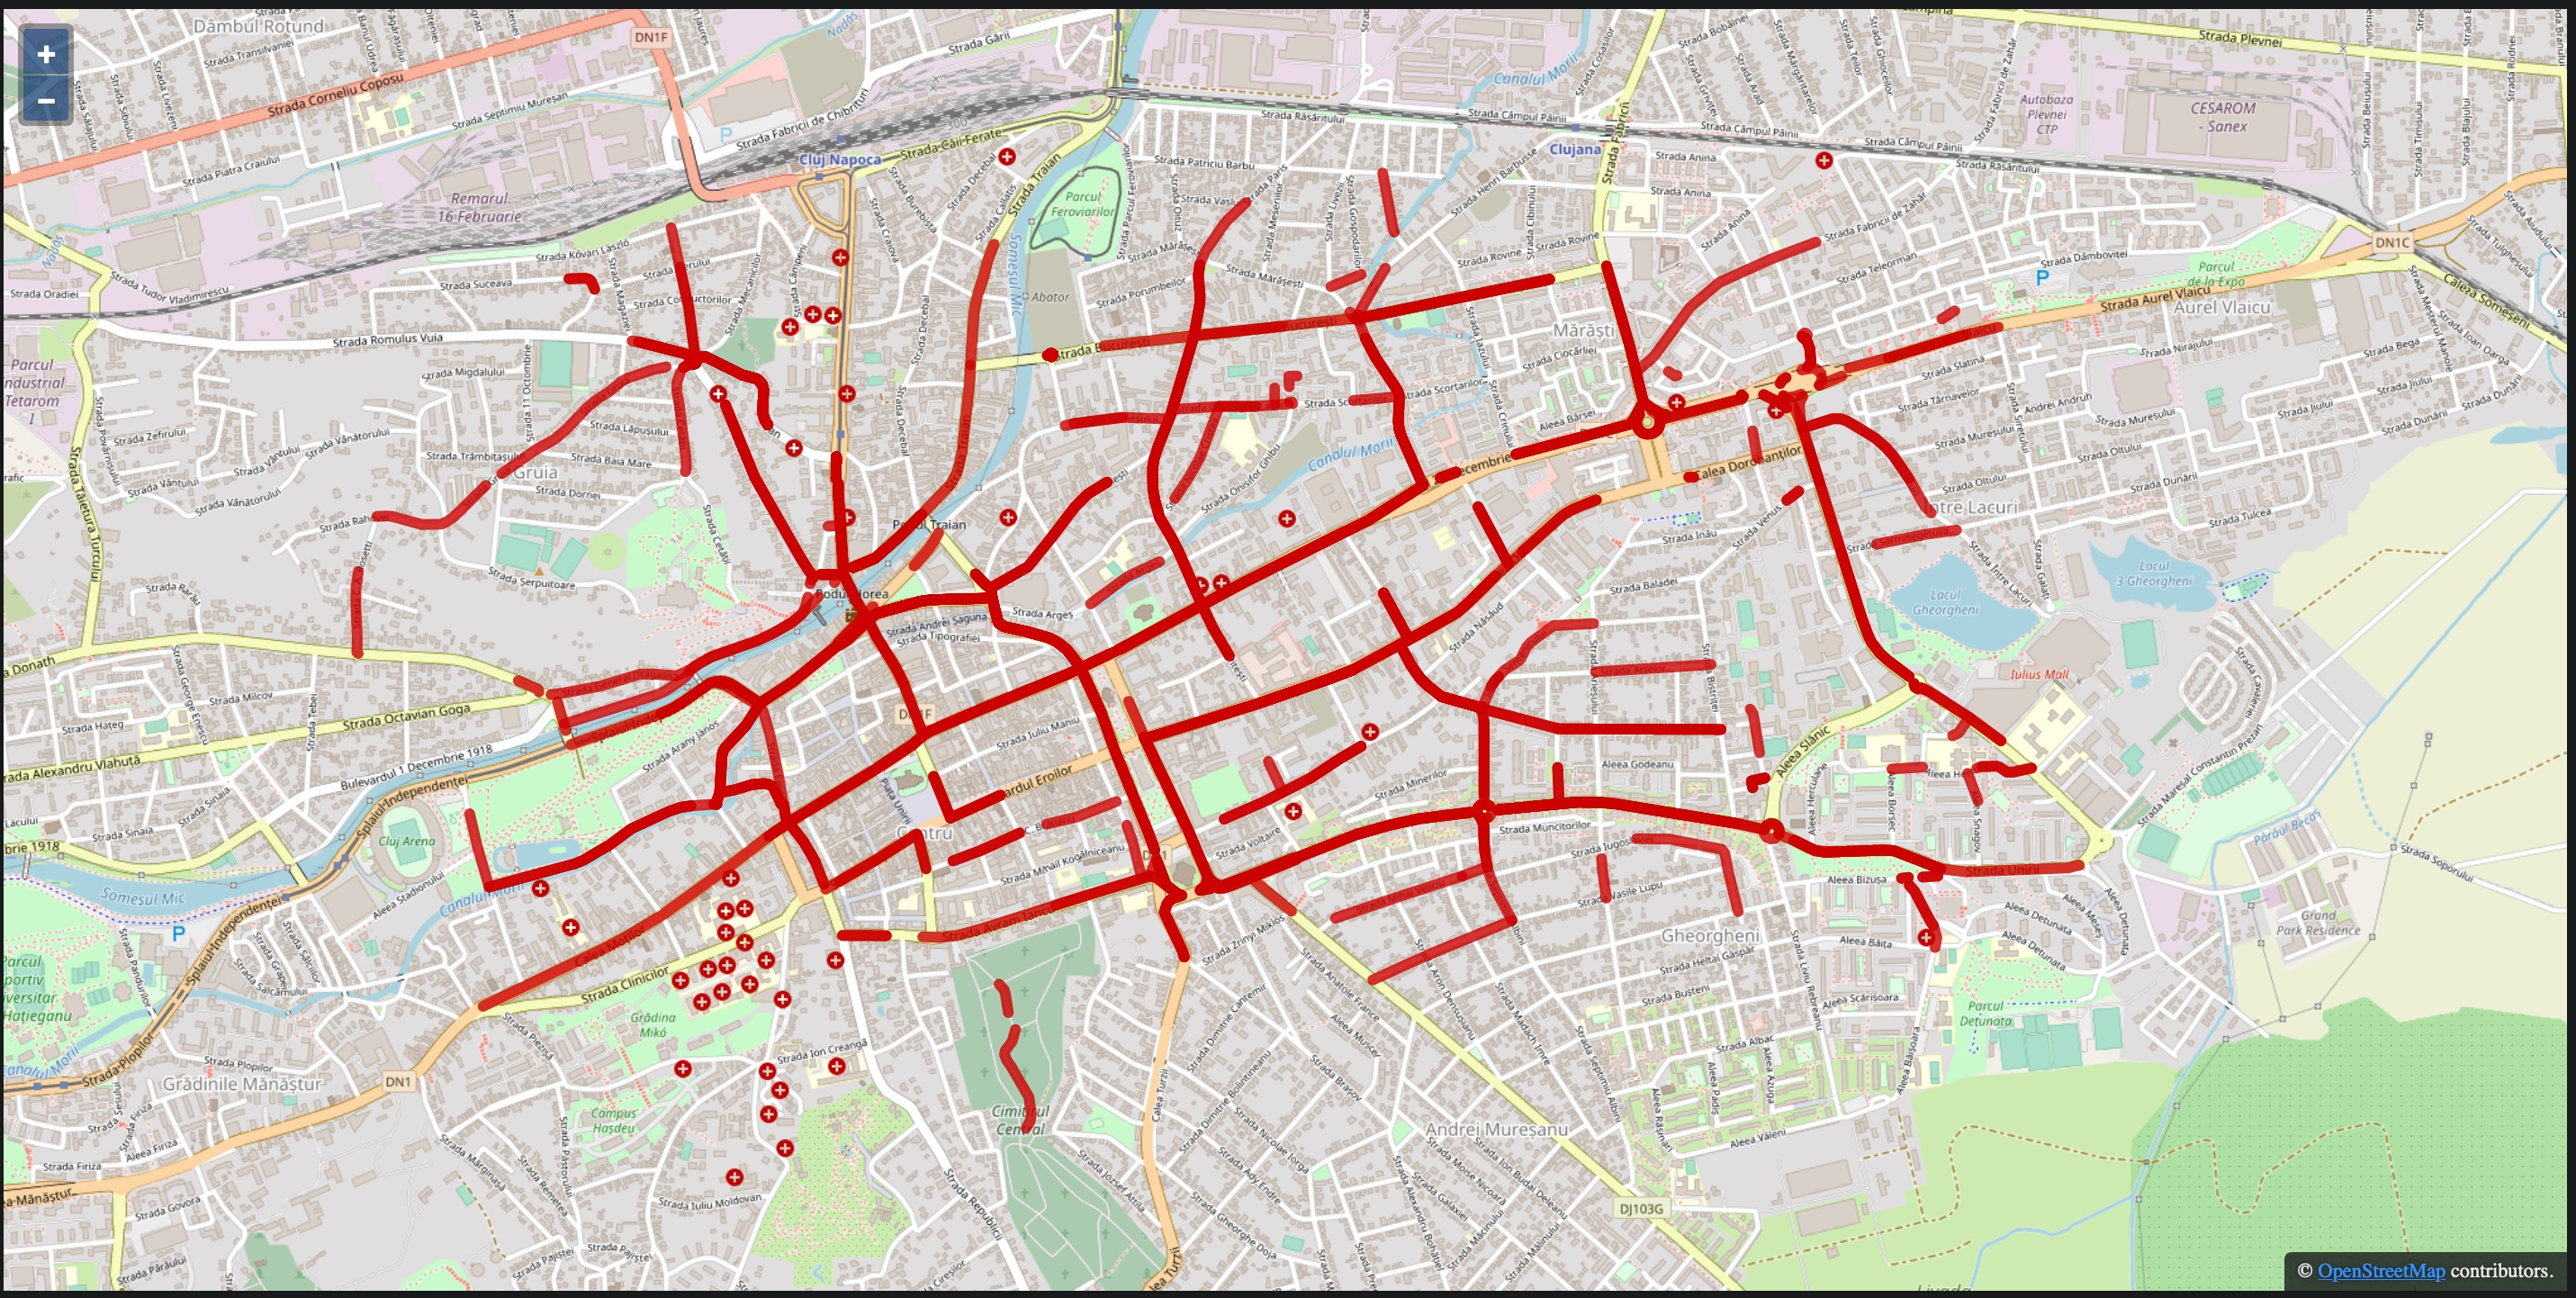
\includegraphics[width=0.9\linewidth]{ScreenshotWebInterface2.jpg}
    \centering
    \caption{Screenshot of the web interface showing the running simulation}
    \label{fig:ScreenshotWebInterface2}
  \end{figure*}

\section{City traffic optimizations}
\label{sec:citytrafficoptimizations}

\subsection{Actors with different behaviors}
\label{subsec:actordiffbehaviors}

One good opportunity for studying the traffic in a city is to model different actor types, each with different behaviors and travel rules. They all share same common goal: travel a route in as little time as possible. But the means of traveling (car, bus, pedestrian, etc.) and the rules (junctions, sidewalks, stop signs, bus lanes, bicycle lanes, etc.) are different for each of them. Therefore the interaction between them start to be complex in modeling via macro-mathematical means. Three examples are discussed in more detail:

\paragraph{Cars} They are the default example of the current chapter. Their behavior is described in subsection \ref{subsec:citysimulator} and is presented here only as a comparison member for the other examples.
\paragraph{Pedestrians} \label{par:pedestrians} They differ drastically from the cars in few aspects. First is the fact that they do not share same space of a street. From the perspective of a city simulator this means that it needs to know the actor type and it needs to maintain a separate zone of density information. The second aspect is that, altough, the pedestrian are by default walking on bare foots along streets, they might take public transport or taxis to travel between their points of interests. This has to be reflected into their routing algorithms. The other part of this aspect is discussed in subsection \ref{subsec:relationsbetweenactors}.
\paragraph{Buses} Those are the same as cars but they have a fixed travel route to move across. Also they might share same lanes with cars or they might have different lanes. Thus the city simulator needs to know this actor type too and it needs to know where on the map they have special public transport lanes, to keep appropiate density numbers for them.
\paragraph{Bicycles} The interesting particularity of those are the fact that they can limit the speed of other actors (cars or buses) to their speed on the places where overtaking is not possible. Again, this is one more burden for the city simulator because it needs to know where bicycles are and it needs to know which streets are too narrow.

\subsection{Relations between actors}
\label{subsec:relationsbetweenactors}

\paragraph{Driving rules} Those are probably the most common interactions between actors. They interact with one another, regardless of their type, through the way a city works. Such a relation might be modeled by a junction or roundabout. Or it might be a crosswalking. Therefore the city simulator, once again, need to take into account those details. Modeling a junction might not be an easy feat and most probably here lies one of the places where a discrete-computed approach is more difficult to define and implement than an analogic aproximation. The difference, altough stated in loosely defined terms is that the definition of density can be a function of the number of actors on a given street. This can be computed at any time (or, better yet, it is computed on every event which occurs. i.e. an actor reporting its state on or off a street). A junction, to the contrary, might be too dynamic to be easy modeled the same way. An aproximation of it is a coefficient based upon an actor is allowed to go through that junction and continue its journey. Whenever an actor reaches a junction its algorithm will have to compute its advance speed based not only on the density (or speed coefficient) number but also based on the junction coefficient. And, of course, the city simulator might choose to vary that very junction coefficient based on a number of factors such as how many cars are awaiting on a joined street (intuitively, as more and more cars are piling up around a junction, harder it is to pass through it).

\paragraph{Contained actors}
The paragraph \ref{subsec:actordiffbehaviors} discussed a type of actor called pedestrians. They might independent but also they might choose to take a bus from one point to another. We call this a contained actor. Thus its reporting will be enriched with one more detail: if is walking by itself or if its inside a bus or a subway. The city simulator will have to compute the densities accordingly for the street or sidewalk but also it might need to know how many pedestrians is a bus allowed to carry.

\paragraph{Close-follow actors}
The bicycle which pedals onto a bus lane might be holding up a bus behind it. Or a number of cars if it's on a common lane. Therefore the speed they have might not be the one which they have without a bike.

\subsection{Exception situations}
Various situations, altough exceptional, might have a big influence on the surround traffic. If a portion of a street is going under few heavy modifications then the traffic might not be allowed to flow through there. Or if a car is stopped on the lane with hazard lights on. Therefore the city simulator will have the opportunity to modify the speed coefficient. It might choose to make it difficult for traffic to pass through that area (if out of 4 lanes, two for each direction, only 2 are used, one for each direction) or it might choose to completely block the portion. It would be of great interest to see, in this case, how the traffic adapts itself to flow through other streets and how much pressure it puts on them, on a different situation than the usual one. The situation of a completely blocked street might also pose the idea of making it a pedestrian-only street and study the effect it would have on the car traffic.

\subsection{Analyzers}

The final part of this traffic simulation chapter is about the possibilities of analyzing pieces of the big picture. It is the supreme purpose of a traffic simulation, to be able to analyze how it works, what specific behaviors it exhibits, in order to find new means and ways of improving it.

The central piece of those analyzers is the city simulator. It contains all the centralized data, from all its actors and it has a minimal API (Application Programming Interface) to serve this data. Actors are the first to consume it as they might need various pieces of information to wisely choose their track. A separate microservice may be the one which takes this data and analyzes it further. The reason for a separate microservice is the separation of concerns. The city simulator is responsible only for keeping together the data and serving it. Any other duty of transform, extrapolate, etc. is not its task to do.

Therefore few ways of taking advantage of this data are described below. They are by no means exhaustive and represent only few places to start.

\paragraph{Hot areas}

Hot areas are defined as places or streets where traffic is pilling up more than in other areas. Figure \ref{fig:ScreenshotWebInterface2} \citep{microservicestrafficsimulation} shows such a analyze using visual cues: streets are colored with red where there cars on them. A slight implementation of this would be to color them gradually and proportional with how many cars are on a specific street. Therefore the human eye will have a better understanding. Other places which could be analyzed are junctions. Figure \ref{fig:ScreenshotWebInterface2} doesn't show how much load are on junctions or roundabouts but there is an opportunity to take adjacent numbers from the city simulator and compute how much cars are able to pass a certain junction in a given time frame.

\paragraph{Statistics numbers}

Sourcing data from the city simulator can meet other necessities. For example the average speed on a street interval, within a given time interval during the day. This could show how much the traffic is slowing down or speeding up. The dynamics of a street or of a neighborhood can be studied in more detail and with greater accuracy. The cars density can be extrapolated and linked to the emissions they have and their impact on the city atmosphere. The density distribution over time could lead to a better understanding of how the traffic is piling up or down during the day. 

\paragraph{Geographical differences}

Another place where those kind of simulation can be helpful is to study would-be differences in the geography of the city. A junction can be replaced with a roundabout and based on the extrapolated data from the other roundabouts of the city it can be studied what impact this modification might have. There are other modifications which can undergo the same study treatment. One would be to add a new lane or, conversely, to remove a lane and make it for public transport only. A street can be closed to study its impact on the surrounding streets and asses whether a temporary closing is possible or not. Or if it's possible to make it a street only for pedestrians. Or to make it one way. Those are things which can be studied before actual modifications of them and without disturbing a highly loaded city neighborhood.

\bibliography{wiki}

\end{document}
